\section{Results}
\label{sec:results}

\begin{figure}[t]
\begin{center}
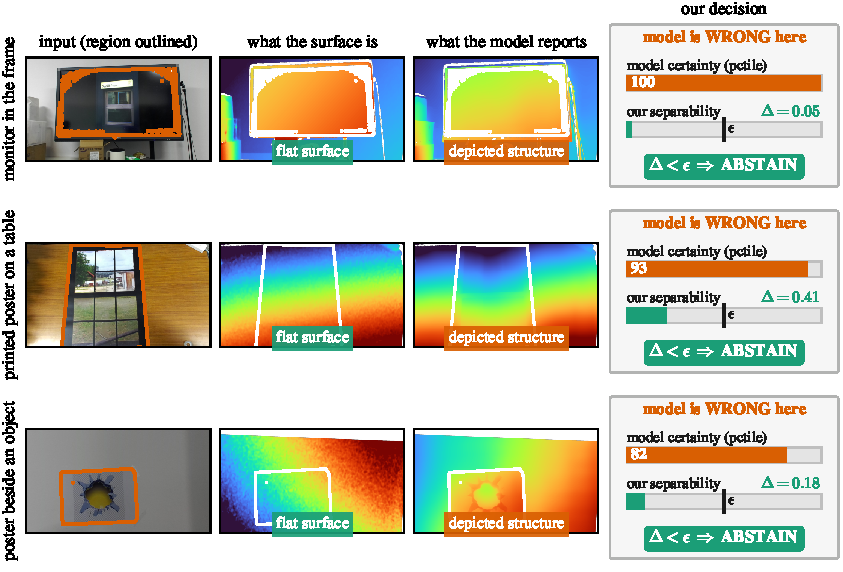
\includegraphics[width=0.88\linewidth]{figures/fig_qualitative.pdf}
\end{center}
\caption{\textbf{Why the decision is needed.} Each row is an image the model gets
wrong: the reference shows a flat sheet or panel, the model reports the structure
depicted on it. Being wrong costs it no certainty, and in the top row it is the
most confident prediction of all $296$ images. The separability $\Delta$ available
from the executed motion falls below $\epsilon$ in every case, so \eqref{eq:abstain}
declines to answer. Across the benchmark $82$ of $296$ images are failures where the
model ranks in the most-confident $30\%$ and this rule abstains.}
\label{fig:qualitative}
\end{figure}

\subsection{Synthetic benchmark}
\label{sec:res-synth}

Table~\ref{tab:phase1} reports Phase~1 over $11$ seeds with the benchmark redrawn
per seed, so intervals reflect the data-generating process rather than model-side
noise. The single-view classifier sits at exactly chance in every seed, confirming
that the matched construction leaves nothing for a single view to exploit, and the
ordering single-view $<$ passive $<$ intervention-aware holds strictly in $11/11$
seeds individually.

\begin{table}[t]
\caption{\textbf{Phase~1, $11$ seeds, mean $\pm$ std, chance $0.333$.} CEA scores
abstention as an error, so committed accuracy is the like-for-like column. Removing
hypothesis conditioning collapses every separability to zero and the system
abstains everywhere, the correct failure mode for a load-bearing component.}
\label{tab:phase1}
\begin{center}
\footnotesize
\begin{tabular}{lccccc}
\toprule
\textbf{Method} & \textbf{CEA} & \textbf{Committed} & \textbf{Abst.} &
\textbf{AUROC} & \textbf{FPCR} \\
\midrule
Single-view classifier    & $0.333{\pm}0.000$ & $0.333{\pm}0.000$ & $0\%$  & $0.505{\pm}0.066$ & $0.000{\pm}0.000$ \\
Passive multi-view        & $0.621{\pm}0.046$ & $0.621{\pm}0.046$ & $0\%$  & $0.748{\pm}0.065$ & $0.868{\pm}0.107$ \\
Generic NBV proxy         & $0.371{\pm}0.050$ & $0.706{\pm}0.029$ & $48\%$ & $0.898{\pm}0.026$ & $0.000{\pm}0.000$ \\
Random intervention       & $0.409{\pm}0.056$ & $0.730{\pm}0.027$ & $44\%$ & $0.925{\pm}0.024$ & $0.000{\pm}0.000$ \\
Max-baseline intervention & $0.502{\pm}0.061$ & $0.824{\pm}0.019$ & $39\%$ & $0.963{\pm}0.028$ & $0.000{\pm}0.000$ \\
\midrule
\emph{abl.}\ no hypothesis cond. & $0.000{\pm}0.000$ & --- & $100\%$ & $0.500{\pm}0.000$ & $0.000{\pm}0.000$ \\
\emph{abl.}\ noisy encoder       & $0.557{\pm}0.034$ & $0.848{\pm}0.049$ & $34\%$ & $0.994{\pm}0.016$ & $0.008{\pm}0.026$ \\
\emph{abl.}\ no abstention       & $\mathbf{0.722{\pm}0.029}$ & $0.722{\pm}0.029$ & $0\%$ & $1.000{\pm}0.000$ & $0.832{\pm}0.107$ \\
\textbf{Ours} & $0.560{\pm}0.032$ & $\mathbf{0.855{\pm}0.054}$ & $34\%$ & $1.000{\pm}0.000$ & $\mathbf{0.000{\pm}0.000}$ \\
\bottomrule
\end{tabular}
\end{center}
\end{table}

Table~\ref{tab:phase2} isolates the choice of intervention. In both studies the
summed objective \eqref{eq:sum} falls short on mirrors while maximin
\eqref{eq:maximin} reaches $1.000$, because a belief-weighted sum can be maximised
by an action that separates pairs not in contention and leaves the deciding pair
unseparated. The gap is structural rather than a threshold choice, since an action
scoring zero on a pair cannot separate it at any $\epsilon$.

\begin{table}[t]
\caption{\textbf{Choosing the intervention, $11$ seeds per study.} Under forced
choice maximin exceeds the passive baseline by $+0.297$ ($t = 41.6$, $11/11$
seeds). Chance is $0.250$ in Phase~2.}
\label{tab:phase2}
\begin{center}
\footnotesize
\begin{tabular}{lccccc}
\toprule
& \multicolumn{2}{c}{\textbf{Mirror committed}} &
\multicolumn{3}{c}{\textbf{Phase~2, four mechanisms}} \\
\cmidrule(lr){2-3}\cmidrule(lr){4-6}
\textbf{Objective} & selector study & Phase~2 & committed & abstains & forced CEA \\
\midrule
Single-view classifier & --- & --- & $0.250{\pm}0.000$ & $0\%$ & $0.250{\pm}0.000$ \\
Passive multi-view     & --- & --- & $0.510{\pm}0.021$ & $0\%$ & $0.510{\pm}0.021$ \\
Max-baseline           & --- & $0.887$ & $0.930{\pm}0.019$ & $73\%$ & --- \\
Summed \eqref{eq:sum}  & $0.587{\pm}0.172$ & $0.956{\pm}0.037$ & $0.986{\pm}0.011$ & $69\%$ & --- \\
\textbf{Maximin} \eqref{eq:maximin} & $\mathbf{1.000{\pm}0.000}$ & $\mathbf{1.000{\pm}0.000}$ & $\mathbf{1.000{\pm}0.000}$ & $72\%$ & $\mathbf{0.808{\pm}0.024}$ \\
\bottomrule
\end{tabular}
\end{center}
\end{table}

\subsection{Real photographs}
\label{sec:res-universal}

Twelve published checkpoints spanning six architecture families and a $38\times$
range in parameter count are evaluated as released
(Figure~\ref{fig:main}a,b; per-checkpoint values in Table~\ref{tab:models}). Every
one is fooled on $59.5$--$78.4\%$ of admissible images, the newest family among the
most affected, and on every one the model's own confidence scores below chance at
predicting its own failure ($0.234$--$0.465$), while identifiability ranges
$0.467$--$0.719$ and exceeds confidence on all twelve.

Calibration cannot repair a signal ordered against the quantity of interest. Both
signals meet their split-conformal coverage guarantee at all five levels tested,
yet deferring on confidence leaves a retained set failing at $76.6\%$ against a
$65.2\%$ base rate, while deferring on identifiability lowers it to $54.4\%$
(Figure~\ref{fig:main}d, Table~\ref{tab:conformal}).

\begin{figure}[!htb]
\begin{center}
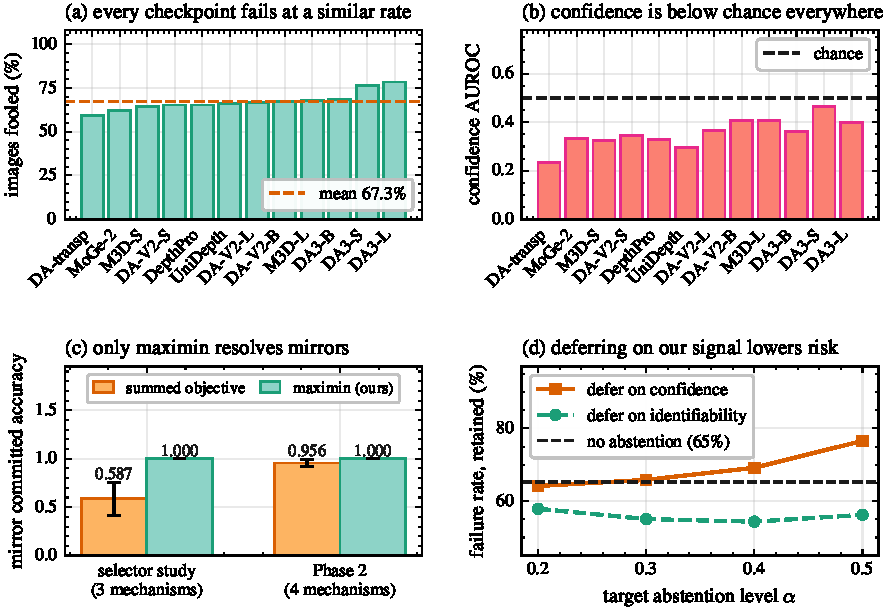
\includegraphics[width=\linewidth]{figures/fig_main.pdf}
\end{center}
\caption{\textbf{Headline results.} (a) The proportion of images each checkpoint is
fooled on stays within a narrow band despite a $38\times$ range in parameter count,
so the behaviour is structural rather than a capacity limitation. (b) Every
checkpoint's own confidence lies below chance at predicting its own failure.
(c) Mirror committed accuracy in both selector studies; only maximin reaches
$1.000$. (d) Split-conformal selective risk: both signals meet coverage, but only
deferring on identifiability lowers the failure rate.}
\label{fig:main}
\end{figure}

Two further measurements support the protocol. The admissibility criterion of
Section~\ref{sec:real-protocol} excludes $159$ of $455$ images whose stereo
reference locks onto displayed content rather than the panel; on admissible images
where a monitor fills the frame, error inside the region is $2.22\times$ that
outside and every image is fooled, with reference planarity $0.989$ against $0.821$
for the prediction. Independently, on a second dataset with ordinal rather than
dense supervision, accuracy split by the benchmark authors' own per-point layer
index gives $0.848$ against $0.737$ across $306{,}874$ pairs, and a second
architecture shows a larger gap still ($0.843$ against $0.669$;
Table~\ref{tab:supp-layered}). That label shares no machinery with any measure
defined here.

\subsection{Choosing where to look, on real photographs}
\label{sec:res-viewpoint}

The benchmark photographs each static scene from several camera positions, and the
median stereo disparity differs across those frames while the scene itself does
not, which is what a moved observer produces. Fifty-five scenes therefore offer a
real action set of three or more viewpoints, and selection can be evaluated on
photographs rather than in simulation. Applying
\eqref{eq:evidence-selection}, and measuring the relative error inside the
ambiguous region so that the outcome depends on no other part of the image,
choosing the best-explained viewpoint reduces that error by $\mathbf{31.6\%}$
relative to choosing uniformly at random, and does so on $\mathbf{12}$ of $12$
checkpoints; the proportion of images on which the predictor is fooled falls from
$48.7\%$ to $44.1\%$, on $9$ of $12$. Table~\ref{tab:supp-viewpoint} gives the full
comparison. What is measured is the error at the chosen viewpoint rather than the
recovery of the mechanism itself, since real images carry no mechanism annotation;
it is the closest test the data supports.

\subsection{Learned abstention}
\label{sec:res-learned}

The signals above are hand-designed, so a natural question is whether a learned
combination does better and whether what it learns is specific to one predictor.
Under leave-one-model-out, a gradient-boosted policy trained on eleven checkpoints
and tested on the twelfth reaches $\mathbf{0.880}$ against $0.764$ for the
strongest single feature, ahead on $\mathbf{12}$ of $12$ held-out checkpoints
(Figure~\ref{fig:transfer}). Nested selection moves that by under $0.01$ and two
boosted families agree within $0.002$, so it is not an artefact of tuning. On a
single checkpoint, where every method sees identical data, a head reading
\emph{frozen} encoder features reaches $\mathbf{0.879}$ against $0.858$ for ten
hand-designed quantities and $0.819$ for the strongest single feature
(Table~\ref{tab:supp-learned}).


